% !TEX TS-program = pdflatex
% !TEX encoding = UTF-8 Unicode

% This is a simple template for a LaTeX document using the "article" class.
% See "book", "report", "letter" for other types of document.

\documentclass[11pt]{scrartcl} % use larger type; default would be 10pt

\usepackage[utf8]{inputenc} % set input encoding (not needed with XeLaTeX)

%%% Examples of Article customizations
% These packages are optional, depending whether you want the features they provide.
% See the LaTeX Companion or other references for full information.

%%% PAGE DIMENSIONS
\usepackage{geometry} % to change the page dimensions
\geometry{a4paper} % or letterpaper (US) or a5paper or....
% \geometry{margin=2in} % for example, change the margins to 2 inches all round
% \geometry{landscape} % set up the page for landscape
%   read geometry.pdf for detailed page layout information

\usepackage{graphicx} % support the \includegraphics command and options

% \usepackage[parfill]{parskip} % Activate to begin paragraphs with an empty line rather than an indent

%%% PACKAGES
\usepackage{booktabs} % for much better looking tables
\usepackage{array} % for better arrays (eg matrices) in maths
\usepackage{paralist} % very flexible & customisable lists (eg. enumerate/itemize, etc.)
\usepackage{verbatim} % adds environment for commenting out blocks of text & for better verbatim
\usepackage{subfig} % make it possible to include more than one captioned figure/table in a single float
\usepackage{float}
\usepackage{listings}
\usepackage{amssymb}


% These packages are all incorporated in the memoir class to one degree or another...

%%% HEADERS & FOOTERS
\usepackage{fancyhdr} % This should be set AFTER setting up the page geometry
\pagestyle{fancy} % options: empty , plain , fancy
\renewcommand{\headrulewidth}{0pt} % customise the layout...
\lhead{}\chead{}\rhead{}\lhead{}\chead{\textit{CS27020 Assignment: Ski Lifts and Pistes : jee22}}\rhead{}
\lfoot{\textit{Aberystwyth University}}\cfoot{\thepage}\rfoot{\textit{Computer Science}}

%%% SECTION TITLE APPEARANCE
\usepackage{sectsty}
\allsectionsfont{\sffamily\mdseries\upshape} % (See the fntguide.pdf for font help)
% (This matches ConTeXt defaults)

%%% ENVIRONMENT ITEMIZE
\newenvironment{myitemize}
{ \begin{itemize}[]
    \setlength{\itemsep}{0pt}
    \setlength{\parskip}{0pt}
    \setlength{\parsep}{0pt}     }
{ \end{itemize}                  } 

%%% LISTINGS LANGUAGE
\lstset{language=SQL}

%%% ToC (table of contents) APPEARANCE
\usepackage[nottoc,notlof,notlot]{tocbibind} % Put the bibliography in the ToC
\usepackage[titles,subfigure]{tocloft} % Alter the style of the Table of Contents
\renewcommand{\cftsecfont}{\rmfamily\mdseries\upshape}
\renewcommand{\cftsecpagefont}{\rmfamily\mdseries\upshape} % No bold!

%%% END Article customizations

%%% The "real" document content comes below...

\title{Brief Article}
\author{The Author}
%\date{} % Activate to display a given date or no date (if empty),
         % otherwise the current date is printed 

\begin{document}
\newpage

\begin{center}
\textbf{\LARGE CS27020}\\[0.3cm]
\textbf{\LARGE Modelling Persistent Data}\\[0.5cm]
\textbf{\LARGE Assignment: Ski Lifts and Pistes }\\[13cm]

\begin{tabular}{ l | r }
{\large Author:} & {\large Address:} \\
James Euesden (jee22) &  Department of Computer Science \\
 & Aberystwyth University \\ 
 & Aberystwyth \\
 & Ceredigion \\
 & SY23 3DB \\
{\large Date:} \today  &  \\

\end{tabular} \\[0.2cm]

{\small Copyright © Aberystwyth University 2014}

\end{center}

%%%\newpage

%%%\tableofcontents

\newpage

\section{Introduction}
The task set for this assignment was to build a relational database, using PostgreSQL, based upon Pistes and Lifts. To begin this task, I was provided with sample data of Pistes and Lifts, which must be viewed in Unnormalized Form (UNF), and then taken through the normalization process to reach Third Normal Form (3NF). This had to be done by determining the Functional Dependencies, selecting Primary Keys and Candidate Keys, then using these to help with the normalization steps.

With the resulting model, I then had to create an appropriate database in PostgreSQL. Provided with the sample data was a number of queries requests that had to be written. These queries had to show the database working, and evidence of their correct operation would support the design and functional dependencies determined in my analysis. The evidence of this testing was to be provided in a series of screenshots and typescripts of the SQL commands.

\section{Analysis}
\subsection{Unnormalized Structure}
An Unnormalized Structure/Form (UNF) is data that has not yet been Normalized, or ready to be put safely and logically into a relational database. This is data that we might find in the 'real world', during situations where we are provided large quantities of data that, while it might make logical sense to a client, may not be appropriate to be implemented into a relational database and cause issues during use.

The sample data provided\cite{sample} involed the attributes of Pistes, and Lifts that serviced those Pistes. Each of these items had attributes about them, and are displayed in my UNF below. A thing I initially noted is how there appeared to be some correlation between the data in 'rise' in Lift and 'fall' in Piste. However, this only happens for a few of the entries, and often occurs where there are multiple values in records, leaving no true connection between these two.\\[0.3cm]
The UNF Data:

\subsubsection{Piste}
Piste (piste\_name)\newline
Grade (grade)\newline
Length(Km) (length\_km)\newline
Fall (m) (fall\_m)\newline
Lifts (lift\_name)\newline
Open? (piste\_open)

\subsubsection{Lift}
Lift (lift\_name)\newline
Type (lift\_type)\newline
Summit (m) (summit\_m)\newline
Rise (m) (rise\_m)\newline
Length (m) (length\_m)\newline
Operating (operating)

\subsection{Functional Dependencies}
A functional dependency is where data depends upon another piece of data in order to be determined. This can be expressed as FD: X -\textgreater \space Y. If we know what 'X' is, we can find out the value of 'Y' from it. To see the functional dependencies, I made a number of assumptions about the data, based upon the sample data provided.
\subsubsection{Piste}
\textbf{piste\_name -\textgreater \space grade, length\_km, fall\_m, piste\_open}
\\[0.1cm]
We assume that the data describing a Piste (grade, length, fall and open) are functionally dependant upon the piste\_name, and this is how it should be accessed. Each attribute provides a 'fact' about the Piste, based on the piste\_name.\\[0.1cm]
\textbf{piste\_name -\textgreater \space lift\_name}
\\[0.1cm]
In order to find the name of Lifts (lift\_name) servicing a Piste, we must know the piste\_name. However, it should be noted that Lift is in itself it's own relation. On top of this, a Lift can serve many Pistes (Many-to-Many), and so it should be noted that this could also be expressed as:\\[0.1cm]
\textbf{piste\_name -\textgreater \space lift\_name}\\
\textbf{lift\_name -\textgreater \space piste\_name}\\
Where we can find the Pistes connected to a Lift, or the Lifts servicing a Piste. This does not come into effect until our Normalization process however. It should be noted now though, for use later.

\subsubsection{Lift}
\textbf{lift\_name -\textgreater \space lift\_type, summit\_m, rise\_m, length\_m, operating}
\\[0.2cm]
Similar to Piste, we assume that the data about a Lift is functionally dependant upon lift\_name. Each of these items is functionally dependant on the lift\_name, and gives data, a 'fact', about a Lift. If we know the name of a Lift, we can get the other data associated with it.

\subsection{Primary \& Candidate Keys}
A Primary Key (PK) is a key that is unique to each record in a relation, and that will never be repeated in the data set. This key can be a single attribute, or a composite key, comprised of multiple attributes. This key is used as the unique identifier of a relation. When picking a Primary Key, it must conform to being unique to that relation, while also being as unchaging as possible (immutable - could change, but shouldn't).

When deciding the Primary Keys for these relations, I found it challenging to decide the correct course of action. My initial thought was to use the piste\_name and lift\_name. However, while these are likely to be unique, it is also possible that in the future a user may want to change or update the names, causing potential update issues. With this in mind, my choice was to make an auto-incremented integer value for both Piste and Lift in order to represent a Unique Identification number. These are Piste(piste\_uid) and Lift(lift\_uid).

This choice to use a UID means that a user has the freedom of adding a number of different unique Pistes and Lifts, while still giving them the ability to alter the names at a later date. With this considered, I decided to continue using piste\_name and lift\_name as Candidate Keys. This means that while they are not the true Primary Key, they are a Candidate for it, and it should be noted along with the functional dependencies when running the normalization process.

It could now be considered that piste\_name and all it's functionally dependant attributes are now all functionally dependent upon piste\_uid, and the same applies for Lift:\\[0.3cm]
\textbf{piste\_uid -\textgreater \space piste\_name}\\
\textbf{piste\_name -\textgreater \space grade, length\_km, fall\_m, piste\_open}\\[0.3cm]
\textbf{lift\_uid -\textgreater \space lift\_name}\\
\textbf{lift\_name -\textgreater \space lift\_type, summit\_m, rise\_m, length\_m, operating}\\[0.3cm]
\textbf{piste\_uid -\textgreater \space lift\_uid}\\
\textbf{lift\_uid -\textgreater \space piste\_uid}
\\[0.3cm]
These new UIDs will affect our normalization process slightly, but as it can be seen, the attributes have not changed much from the originally found functional dependencies.

As an extra precaution when creating the database, I will constrain the lift\_name and piste\_name to be unique, enforcing the rule that no two Pistes or Lifts should be named the same, but their names are free for change.

\newpage

\section{Normalizing the Data}
As previously mentioned, Normalizing data is the process of working through 'Normalization steps' to reach certain forms. These forms are good for use in relational database models, and each form removes some form of issues when implementing the data into a database. For this task, the data will be taken to 3NF.

\subsection{First Normal Form}
The act of taking data from UNF into 1NF is by disallowing attributes to have multiple values. This means that an attribute could not contain two values, such as 2 phone numbers for one person in the same record. In the sample data provided, it can be seen that within 'Piste', there are multiple values in 'lift\_name'. This violates 1NF rule.

In order to solve this, we can move lift\_name out of the Piste and into a new relation, 'Connection'. This new relation contains the Primary Key of Piste and the attribute lift\_name. Piste no longer contains lift\_name, while otherwise staying the same. This brings Piste into 1NF.

Lift does not have any multiple values within it's attributes, nor could it be assigned any in the future. This means that Lift is already in 1NF and does not need anything doing. There are no more sets of multiple values in Lift or Piste, and Connection is also acceptable, at this stage.

The end result of the 1NF operations are below, with the current three relations shown. Those attributes \underline{underlined} represent Primary Key components. Those attributes with an asterisk (*) are foreign keys. These relations still have some anomalies however, that will be dealt with in 2NF.

\subsubsection{Piste}
\underline{piste\_uid}\newline
piste\_name\newline
grade\newline
length\_km\newline
fall\_m\newline
open

\subsubsection{Lift}
\underline{lift\_uid}\newline
lift\_name\newline
lift\_type\newline
summit\_m\newline
rise\_m\newline
length\_m\newline
operating

\subsubsection{Connection}
\underline{piste\_uid*}\newline
lift\_name*\\[0.3cm]
(Foreign key piste\_uid* references piste\_uid from relation Piste)\\
(Foreign key lift\_name* references lift\_name from relation Lift)

\subsection{Second Normal Form}
Achieving Second Normal Form relies upon two things, the first being that 1NF is already achieved, the second being that every non-Primary Key attribute of the relation is dependent on the whole of a candidate key. As we can see from the new relation 'Connection', lift\_name is not wholly dependent upon 'piste\_uid'. It is dependent upon lift\_uid in the functional dependencies.

With this in mind, the structure of Connections should instead be representing a Many-to-Many relationship, with a full Primary Key comprised of the two foreign keys 'piste\_uid' and 'lift\_uid', and removing lift\_name from 'Connections' entirely.

This results in no non-key attributes within Connections, and the Primary Key UIDs supporting the link between Lift and Piste. The three relations now only have non-key attributes that do solely rely upon the Candidate Keys, and all are valid for 2NF.\\[0.3cm]
The new form of the relations now looks like this:

\subsubsection{Piste}
\underline{piste\_uid}\newline
piste\_name\newline
grade\newline
length\_km\newline
fall\_m\newline
open

\subsubsection{Lift}
\underline{lift\_uid}\newline
lift\_name\newline
lift\_type\newline
summit\_m\newline
rise\_m\newline
length\_m\newline
operating

\subsubsection{Connection}
\underline{piste\_uid*}\newline
\underline{lift\_uid*}\\[0.3cm]
(Foreign key piste\_uid* references piste\_uid from relation Piste)\\
(Foreign key lift\_uid* references lift\_uid* from relation Lift)

\subsection{Third Normal Form}
For a database to be valid for Third Normal Form, it must first conform to 2NF, and also have no transitive dependencies. A transitive dependencies is where an attribute relies on only partial of the Primary Key. It can be described that all non-key attributes rely upon only the PK, and nothing but the PK, providing a fact about the PK and nothing else. 

If we look at our current relations, we can see that this is already the case, where each attribute of data provides a fact about the PK.

Each attributes relies soley upon the Primary Key of its relation, and provides a fact about that whole Primary Key, providing no information about any other aspect of the database or of itself. From all this, we can see that Lift has been in 3NF throughout the whole process, and the database structure does not need to change further. The structure is now in 3NF.

\newpage

\section{PostgreSQL}
With the data now in 3NF, it is suitable to be put into a database. For this task, it must be placed into a PostgreSQL table. I have created this on my personal filestore at Aberystwyth University. Below are the typescripts of the commands I used to create these, and screenshots to demonstrate their use and the results of my queries.

\subsection{Creating the tables}
The typescript for creating the database:

\lstinputlisting[language=SQL]{../SQL/create.sql}

\begin{figure}[H]
  \centering
    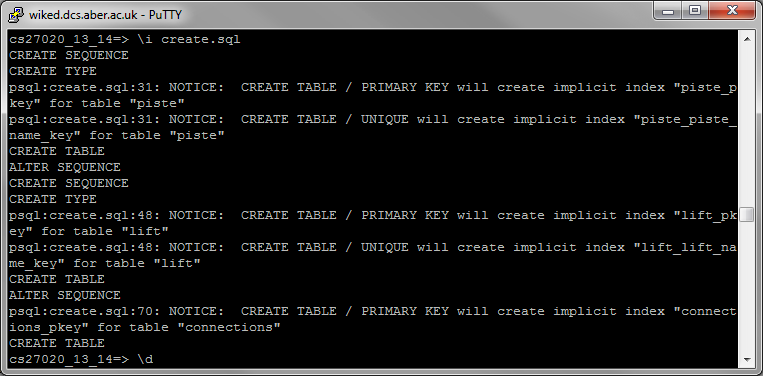
\includegraphics[width=1\textwidth]{IMG/create_tables.png}
 \caption{The output when creating tables.}
\end{figure}
\begin{figure}[H]
  \centering
    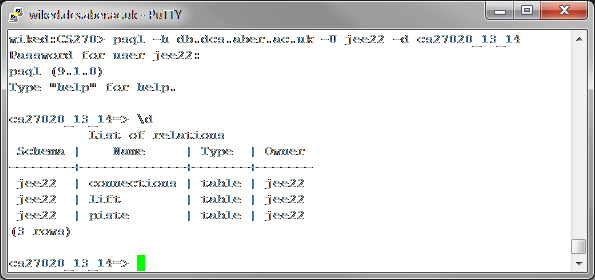
\includegraphics[width=1\textwidth]{IMG/completed_tables.png}
 \caption{The list of relations after running the create typescript.}
\end{figure}

\subsection{Data Types Justification}
For each of the attributes, I carefully selected particular data types that I felt would best represent them. On each data type, I have constrained the type or amount of data that they can take in order to reduce the potential for issues in the databases use. I feel confident in my choices for data types in that they represent the data from the real world as best as they can within my structure.

Most data types have the contraint that they are 'NOT NULL'. When dealing with certain aspects of real data, such as a Piste or Lift, that definitely do have a specfic data, I felt that NOT NULL should be included. There are no items in the sample data that have empty values for attributes. I felt that having the majority of attributes constrain to not null ensures that data is correctly input into the table, avoiding potential issues with updates and missing data for future users. This helps to ensures the integrity of the data throughout it's lifetime.

For those attributes which are numbers, I have also chosen to constrain them to being greater than 0. Doing this stops a user from being allowed to enter negative values. Each of these has also been named using the CONSTRAINT command, in order to better inform the user of where their error lies, such as 'rise\_must\_be\_positive'. These help a user who may have made a slight typing error see where they have gone wrong in an informative error message.
\subsubsection{Piste Data Types}
\begin{itemize}
\item piste\_uid - int NOT NULL\\
The piste\_uid is kept as an integer to be a Unique Identification number. This way of using an integer allows it to be incremented for the number of records entered.
\item piste\_name - varchar(50) UNIQUE NOT NULL PRIMARY KEY\\
varchar allows the input of text, so the user can specify the name of the Piste. Setting the limit at 50 allows for a decent amount of characters without allowing unreasonable amounts. By using the constraint 'UNIQUE', it is enforcing the user to never have two of the same named Pistes.
\item grade - grade\_rank NOT NULL\\
I made a custom TYPE of ENUM for grade\_rank, allowing the user to select from the different types of ranks, and using an ENUM allows for future expansion on these grades if necessary. I based the choices of ranks on those provided in the sample data: Easy, Medium, Hard, Difficult.
\item length\_km - real NOT NULL CHECK (length\_km \textgreater \space 0)\\
Using a real allows some floating point precision. Since the km is used to represent the length, where there can be numbers after the decimal, a real seemed appropriate to reprsent this data. Example: 4.5km.
\item fall\_m - integer NOT NULL CHECK (fall\_m \textgreater \space 0)\\
A way to represent the fall as a whole number in meters.
\item open\_piste - boolean NOT NULL\\
Since a piste can either be open or not open, a true/false boolean seemed appropriate to determine either/or.
\end{itemize}

\subsubsection{Lift Data Types}
\begin{itemize}
\item lift\_uid - int NOT NULL\\
The lift\_uid is kept as an integer to be a Unique Identification number. This way of using an integer allows it to be incremented for the number of records entered.
\item lift\_name - varchar(60) UNIQUE NOT NULL\\
varchar allows the input of text, so the user can specify the name of the Lift. Setting the limit at 60 allows for a decent amount of characters without allowing unreasonable amounts. By using the constraint 'UNIQUE', it is enforcing the user to never have two of the same named Lifts.
\item lift\_type - type\_lift NOT NULL\\
I made a custom TYPE of ENUM for lift\_type, allowing the user to select from the types of lift in the sample data, and using an ENUM allows for future expansion on types if necessary. I based the choices of ranks on those provided in the sample data: Gondola, Tow and Chair.
\item summit\_m - integer NOT NULL CHECK (summit\_m \textgreater \space 0)\\
A way to represent the summit as a whole number in meters.
\item rise\_m - integer NOT NULL CHECK (rise\_m \textgreater \space 0)\\
A way to represent the rise as a whole number in meters.
\item length\_m - integer NOT NULL CHECK (length\_m \textgreater \space 0)\\
A way to represent the length as a whole number in meters.
\item operating - boolean NOT NULL\\
Since a lift can either be operating or not operating, a true/false boolean seemed appropriate to determine either/or.
\end{itemize}

The data types from Connection are the same as those that they Reference, and so the justification of there choices is already included. The attributes comprise the Primary Key as Foreign Keys, and are piste\_uid and lift\_uid.

\newpage
\subsection{Checking the Database}
\subsubsection{Sample Data}
In order to test my database, I wrote the sample data provided into a typescript to insert it into the database tables. I will not include the typescript here. However, here are the contents of each relation after the insertion:

\begin{figure}[H]
  \centering
    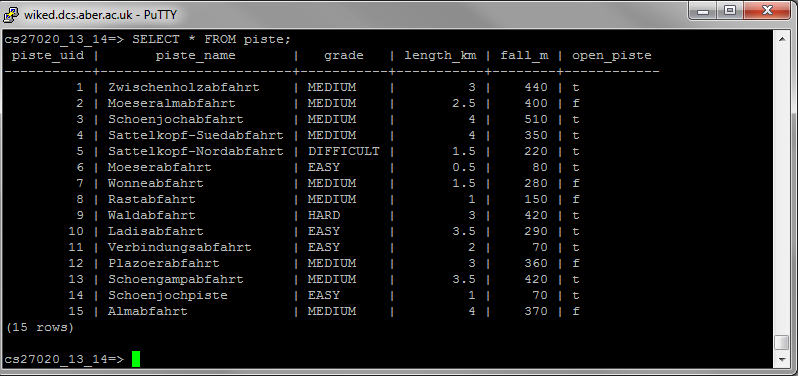
\includegraphics[width=1\textwidth]{IMG/content_piste.png}
 \caption{The contents of the Piste table.}
\end{figure}
\begin{figure}[H]
  \centering
    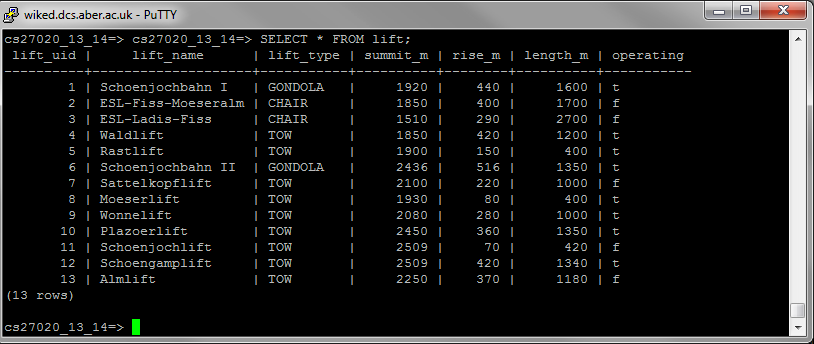
\includegraphics[width=1\textwidth]{IMG/content_lift.png}
 \caption{The contents of the Lift table.}
\end{figure}
\begin{figure}[H]
  \centering
    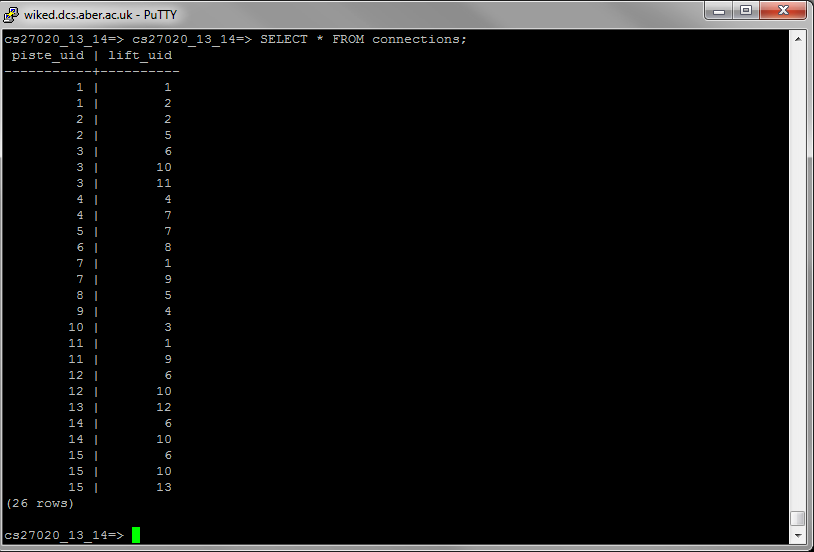
\includegraphics[width=1\textwidth]{IMG/content_connections.png}
 \caption{The contents of the Connections table.}
\end{figure}

\subsubsection{Erronous Data Entry}
In order to check that my database was working correctly, I conducted a series of tests where I attempted to INSERT incorrect data. Doing this confirmed that my database was robust and built as intended. Below are a series of screenshots and captions detailing some my testing.

 I have shown this testing in brief, where I can demonstrate my correctly operating ENUMs, CHECKS and UNIQUE constraints. The ones I have shown are examples, and should be taken as a representation for every other attribute that share the same constraints.

\begin{figure}[H]
  \centering
    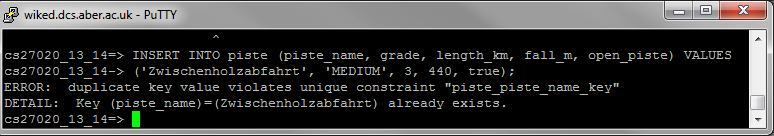
\includegraphics[width=1\textwidth]{IMG/err_exists.png}
 \caption{An entry cannot have the same piste\_name as an already existing Piste - UNIQUE constraint. The item can be renamed, but should not share the same name with another of it's type.}
\end{figure}
\begin{figure}[H]
  \centering
    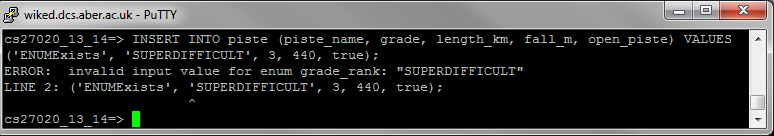
\includegraphics[width=1\textwidth]{IMG/err_no_enum.png}
 \caption{An entered Grade should conform to an existing ENUM value. 'SUPERDIFFICULT' is not an existing ENUM value in this database.}
\end{figure}
\begin{figure}[H]
  \centering
    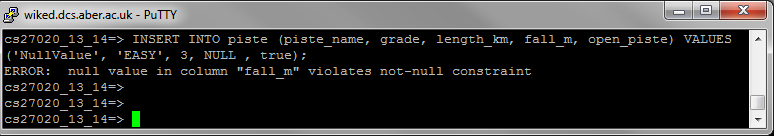
\includegraphics[width=1\textwidth]{IMG/err_null_value.png}
 \caption{If a value is attempted to be entered as NULL, it will be rejected, as values are specific and so should not be recorded into the database as such. This violates the constraint and would potentially cause issues in the databases lifecycle, such as causing errors in queries that might attempt to assess NULL data.}
\end{figure}
\begin{figure}[H]
  \centering
    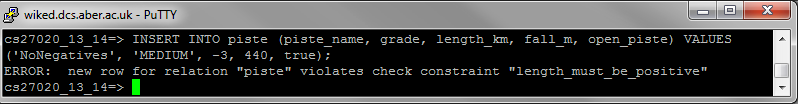
\includegraphics[width=1\textwidth]{IMG/err_no_negatives.png}
 \caption{If a numeric value is attempted to be entered as negative, the operation is cancelled, the user is informed of their mistake and through the use of CONSTRAINT, is told where their mistake is and why. When looking at the sample data, there are no negative numbers. Know what information the data provides shows that there should never be negative values.}
\end{figure}
\newpage

\subsection{Test Queries}
There were 4 queries provided that needed to be successfully carried out in order to test the strucutre of my database:
\begin{itemize}
\item Return the piste(s) served by a given lift
\item Return the lift(s) that provide access to a given piste
\item Return the lifts that are currently operating
\item Return the pistes that are currently open, together with the lifts that are currently operating and that provide access to those pistes
\end{itemize}
It should be noted that where you might see \textless \space and \textgreater in the Test Query typescripts, it should be assumed that here is where a value would go for the query. An example would be '\textless lift\_name\textgreater ' could be imagined to be 'Rastlift', or any other lift\_name, when executing the query.

For queries where it requires multiple queries from multiple tables, I have opted to use 'INNER JOIN', to connect my relations together in order to access the data. I felt that by explicitly stating that I wished to use INNER JOIN, as opposed to having an implied JOIN, was much more robust.

Using the INNER JOIN should improve performance of the database over an implied JOIN, which would be an important factor were the database to be very large. I also feel that using INNER JOIN makes it easier to read as a human than if the queries were comprised of multiple SELECT statements or large lists of data selected from a WHERE clause.
\subsubsection{Test Query 1}
"Return the piste(s) served by a given lift."
\begin{lstlisting}
-- SELECT the Pistes serviced by a particular Lift.
SELECT lifts.lift_name, pistes.*
	FROM piste pistes
		INNER JOIN connections conns
	ON pistes.piste_uid=conns.piste_uid
		INNER JOIN lift lifts
	ON lifts.lift_uid=conns.lift_uid
		AND lifts.lift_name='<lift_name>';
\end{lstlisting}
This query selects all the data concerning the piste(s) that are served by a given lift. The query gets all of the Piste uids from Connections relation which are linked to the Lifts who have uids matching the same uid for the Lift in the Lift relation that share the given lift\_name.

\begin{figure}[H]
  \centering
    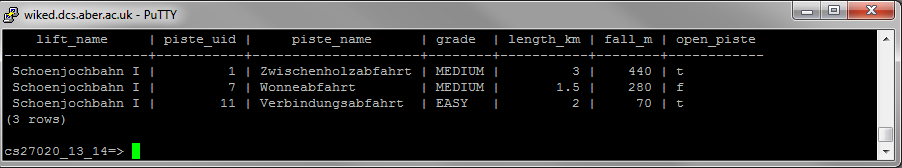
\includegraphics[width=1\textwidth]{IMG/query_1_1.png}
 \caption{The result of looking for the Pistes serviced by the Lift: 'Schoenjochbahn I'.}
\end{figure}

\begin{figure}[H]
  \centering
    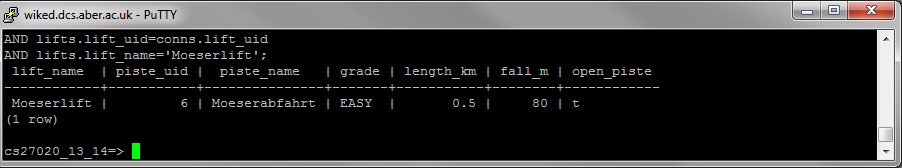
\includegraphics[width=1\textwidth]{IMG/query_1_2.png}
 \caption{The result of looking for the Pistes serviced by the Lift: 'Moeserlift'.}
\end{figure}

\subsubsection{Test Query 2}
"Return the lift(s) that provide access to a given piste."
\begin{lstlisting}
-- SELECT the Lifts that provide access to a given Piste.
SELECT pistes.piste_name, lifts.*
	FROM lift lifts
		INNER JOIN connections conns
	ON lifts.lift_uid=conns.lift_uid
		INNER JOIN piste pistes
	ON pistes.piste_uid=conns.piste_uid
		AND pistes.piste_name='<piste_name>';
\end{lstlisting}
This query is the same as the first query, but looking for Lifts providing access to a particular Piste. The logic for the query is identical forthe first and so should not need to be explained again here.

\begin{figure}[H]
  \centering
    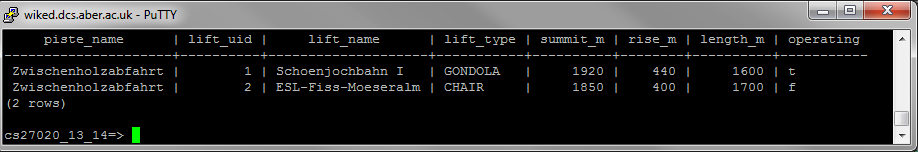
\includegraphics[width=1\textwidth]{IMG/query_2_1.png}
 \caption{The result of looking for the Lifts servicing the Piste: 'Zwischenholzabfahrt'.}
\end{figure}

\begin{figure}[H]
  \centering
    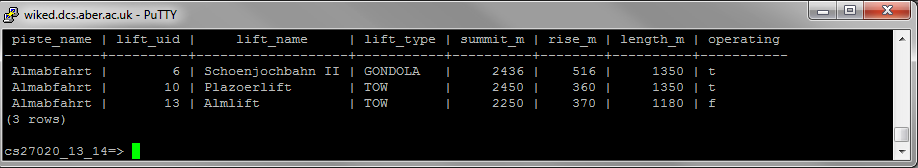
\includegraphics[width=1\textwidth]{IMG/query_2_2.png}
 \caption{The result of looking for the Lifts servicing the Piste: 'Almabfahrt'.}
\end{figure}

\subsubsection{Test Query 3}
"Return the lifts that are currently operating."
\begin{lstlisting}
-- SELECT the Lifts that are currently operating.
SELECT lift_name, operating
	FROM lift WHERE operating='t';
\end{lstlisting}
Look for the Lifts that are currently operating. In this case, look for those that are marked 'TRUE', or 't', in the operating attribute. I chose to only display the lift\_name and it's operational status for this query. However, by exchanging the two requested attributes for an '*', 'SELECT * FROM...', it would return all the data for each of the operating lifts. I also understood the requested query as asking for all Lifts operating, regardless of whether the Pistes they service are open or not.

\begin{figure}[H]
  \centering
    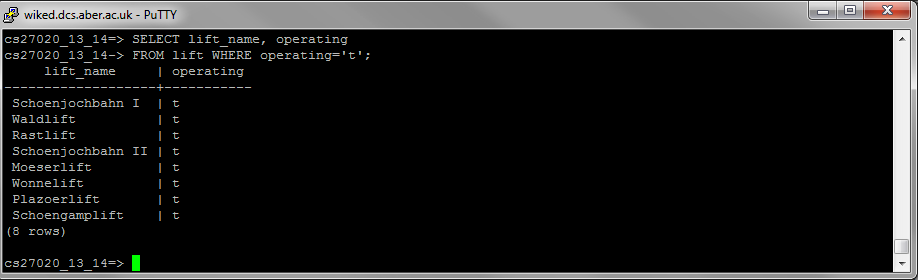
\includegraphics[width=1\textwidth]{IMG/query_3_1.png}
 \caption{The Lifts that are currently operating.}
\end{figure}

%%%%
\newpage
%%%%

\subsubsection{Test Query 4}
"Return the pistes that are currently open, together with the lifts that are currently operating and that provide access to those pistes."
\begin{lstlisting}
-- SELECT the Pistes that are currently open, together with the 
lifts that are currently operating and that provide access to 
those pistes.
SELECT pistes.piste_uid, pistes.piste_name, pistes.open_piste, 
lifts.lift_uid, lifts.lift_name, lifts.operating
FROM
	connections conns
		INNER JOIN piste pistes
	ON pistes.open_piste='t' 
		INNER JOIN lift lifts
	ON lifts.operating='t'
		AND pistes.piste_uid=conns.piste_uid
		AND lifts.lift_uid=conns.lift_uid;
\end{lstlisting}

The final query requests to return all of those Pistes that are currently open. With those Pistes, those listed should also display the Lifts that service them, but only those Lifts that are currently operating. To do this, the query looks for those Pistes that are open, then looks for the Lifts that are also operating, and returns those Lifts that are servicing the open Pistes.

I chose to only return the UIDs, Name and open/operating status of the Pistes and Lifts for the sake of space. As with the previous query, it could easily be modified to provide all data associated with the relevant Lifts and Pistes.

\begin{figure}[H]
  \centering
    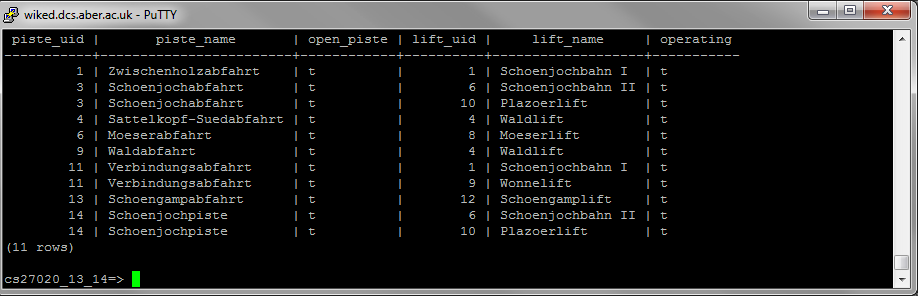
\includegraphics[width=1\textwidth]{IMG/query_4_1.png}
 \caption{The Pistes that are open, with the corresponding connecting Lifts that are currently operating.}
\end{figure}

\section{Conclusion}
With my completed Database, evidence of testing with the sample data, checking for errors and working queries, I feel I have fulfilled the task set. My database correctly takes in the desired data, refusing any data that might violate the conditions or cause future errors, and stores the data in a way that is in 3NF. I have followed the Normalization process to reach 3NF, based on my choices of the Primary/Candidate keys and the functional dependencies. The end result is a fully functional database that could be used for storing data on connected Pistes and Lifts, and queried for the data inside with relative ease.

\newpage
\begin{thebibliography}{9}

\bibitem{sample}
  Edel Sherratt,
  \emph{CS27020 Assignment: Ski Lifts and Pistes}.
  Computer Science Department,
  Aberystwyth University,
  2014.

\end{thebibliography}

\end{document}
